\normaltrue \difficilefalse \tdifficilefalse
\correctionfalse

%\UPSTIidClasse{11} % 11 sup, 12 spé
%\newcommand{\UPSTIidClasse}{11}

\exer{Moteur à courant continu$\star$ \label{B2:07:51}}
\setcounter{numques}{0}
\UPSTIcompetence[2]{B2-07}
\index{Compétence B2-07}
\index{Schéma-blocs}
\index{Moteur à courant continu}
\index{MCC}
\ifcorrection
\else
\textbf{Pas de corrigé pour cet exercice.}
\fi


\ifprof 
\else
On donne les équations du moteur à courant continu :
\begin{itemize}
\item $u(t) = e(t)+ Ri(t) +L \dfrac{\text{d}i(t)}{\text{d} t}$;
\item $e(t)=K\omega(t)$;
\item $c(t)=Ki(t)$;
\item $c(t)- f\omega(t)=J\dfrac{\text{d}\omega(t)}{\text{d} t}$.
\end{itemize}
\fi

\question{Réaliser le schéma-blocs.}
\ifprof
\begin{figure}[H]
\centering
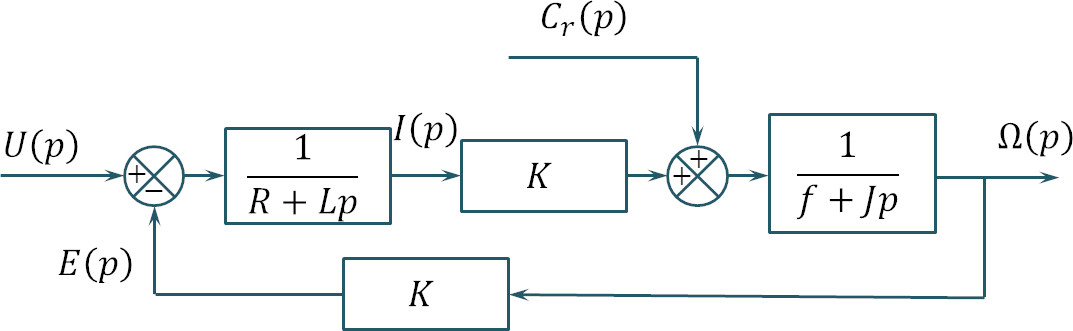
\includegraphics[width=.7\linewidth]{51_01_c}
%\caption{Évolution du couple utile en fonction de la vitesse de rotation pour des
%fréquences de commande de \SI{90}{Hz} à \SI{110}{Hz}. \label{fig_50_04}}
\end{figure}
\else
\fi



\question{Mettre le schéma-blocs sous la forme suivante.}
\ifprof
\begin{figure}[H]
\centering
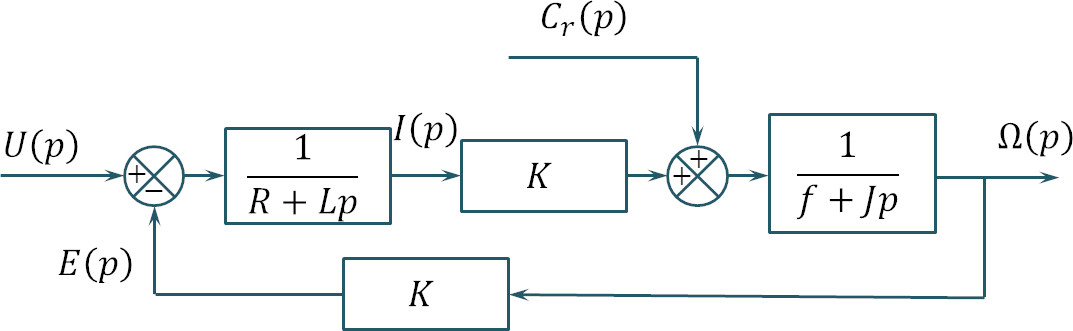
\includegraphics[width=.7\linewidth]{51_01_c}
%\caption{Évolution du couple utile en fonction de la vitesse de rotation pour des
%fréquences de commande de \SI{90}{Hz} à \SI{110}{Hz}. \label{fig_50_04}}
\end{figure}
\else
\begin{figure}[H]
\centering
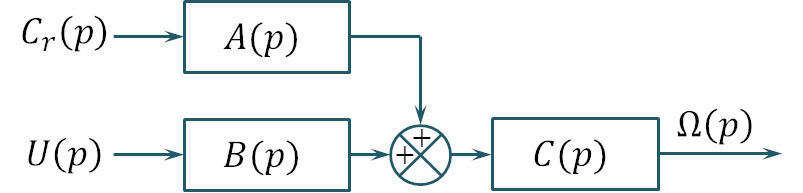
\includegraphics[width=.7\linewidth]{51_01}
%\caption{Évolution du couple utile en fonction de la vitesse de rotation pour des
%fréquences de commande de \SI{90}{Hz} à \SI{110}{Hz}. \label{fig_50_04}}
\end{figure}
\fi





\ifprof
\else
\begin{flushright}
\footnotesize{Corrigé  voir \ref{B2:07:51}.}
\end{flushright}%
\fi